% --------------------------------------------------------------------------------

\begin{exercise}

In einer Menge von $n$ Personen können 10 Personen Deutsch, $9$ Englisch, $9$ Russisch, $5$ Deutsch und Englisch, $7$ Deutsch und Russisch, $4$ Englisch und Russisch, $3$ alle drei Sprachen.
Wie groß ist $n$?

(Hinweis: Prinzip von Inklusion und Exklusion.)

\end{exercise}

% --------------------------------------------------------------------------------

\begin{solution}

\phantom{}

\includegraphicsboxed{Satz 2.1 (Prinzip von Inklusion und Exklusion).png}

\begin{figure}[h!]
  \centering
  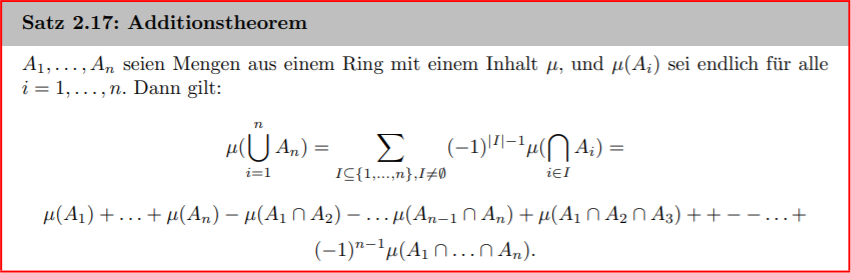
\includegraphics[width = 0.75 \textwidth]{Grill - Maß- und Wahrscheinlichkeitstheorie - Satz 2.17.png}
  \caption{Grill - Maß- und Wahrscheinlichkeitstheorie}
\end{figure}

Wir definieren die Mengen $D, E, R$ jeweils als die Menge aller Deutsch-, Englisch-, Russisch-Sprachler.
Sei $\Omega$ die Menge aller Personen.

\begin{multline*}
  \implies
  |\Omega|
  =
  \underbrace{|(D \cup E \cup R)^C|}_0
  +
  |D \cup E \cup R| \\
  =
  |D| + |E| + |R| - |D \cap E| - |E \cap R| - |R \cap D| + |D \cap E \cap R|
  =
  10 + 9 + 9 - 5 - 7 - 4 + 3
  =
  15
\end{multline*}

\end{solution}

% --------------------------------------------------------------------------------
